% ==========================================================
% PneumoFusionNet — IEEE Conference Paper
% Author: Ashutosh Yadav, IIT Guwahati
% ==========================================================
\documentclass[conference]{IEEEtran}
\IEEEoverridecommandlockouts

% ── Core packages ─────────────────────────────────────────
\usepackage{cite}
\usepackage{amsmath,amssymb,amsfonts}
\usepackage{algorithmic}
\usepackage{graphicx}
\usepackage{textcomp}
\usepackage[utf8]{inputenc}
\usepackage[T1]{fontenc}
\usepackage{hyperref}
\usepackage{url}
\usepackage{booktabs}
\usepackage{nicefrac}
\usepackage{microtype}
\usepackage{multirow}
\usepackage{enumitem}
\usepackage{subcaption}
\usepackage{tcolorbox}
\tcbuselibrary{skins}

% ── AI Colour Palette ────────────────────────────────────
\usepackage{xcolor}
\definecolor{aideep}{RGB}{26, 35, 126}       % Deep AI indigo
\definecolor{aiaccent}{RGB}{0, 150, 136}      % Teal accent
\definecolor{aiwarm}{RGB}{255, 87, 34}        % Warm orange
\definecolor{aicyan}{RGB}{0, 188, 212}        % Cyber cyan
\definecolor{aipurple}{RGB}{156, 39, 176}     % Neural purple
\definecolor{aigreen}{RGB}{76, 175, 80}       % Success green
\definecolor{aigold}{RGB}{255, 193, 7}        % Attention gold
\definecolor{aisoft}{RGB}{232, 234, 246}      % Soft lavender bg
\definecolor{aitextblue}{RGB}{13, 71, 161}    % Dark blue text
% ── Hyperlink styling ────────────────────────────────────
\hypersetup{
  colorlinks=true,
  linkcolor=aideep,
  citecolor=aiaccent,
  urlcolor=aiaccent
}

\def\BibTeX{{\rm B\kern-.05em{\sc i\kern-.025em b}\kern-.08em
    T\kern-.1667em\lower.7ex\hbox{E}\kern-.125emX}}

\begin{document}

% ==========================================================
%  TITLE
% ==========================================================
\title{\textcolor{aideep}{PneumoFusionNet: Multimodal Pneumonia Detection via Chest X-Ray, Radiology Text, and White Blood Cell Fusion}}

\author{
\IEEEauthorblockN{Ashutosh Yadav}
\IEEEauthorblockA{
\textit{Mehta Family School of Data Science and Artificial Intelligence} \\
\textit{Indian Institute of Technology Guwahati, India}\\
Assam, India \\
ashutosh.yadav@op.iitg.ac.in
}
}

\maketitle

% ==========================================================
%  ABSTRACT
% ==========================================================
\begin{abstract}
\begin{tcolorbox}[
  colback=aisoft!70,
  colframe=aideep,
  arc=3pt,
  boxrule=0.8pt,
  left=5pt,right=5pt,top=5pt,bottom=5pt
]
\noindent\textbf{\textcolor{aideep}{Clinical Problem:}} \textbf{Chest radiography (CXR) interpretation is constrained by severe visual overlap with atelectasis and non-infectious opacities, while imaging alone cannot quantify host systemic inflammation.}

\vspace{3pt}
\noindent\textbf{\textcolor{aideep}{Multimodal Approach:}} \textbf{We present PneumoFusionNet, evaluated on 3{,}763 frontal posteroanterior radiographs from MIMIC-CXR coupled with clinical notes and laboratory records from MIMIC-IV. The framework integrates a DenseNet-121 backbone (with CBAM attention) and Bio\_ClinicalBERT token representations via 8-head cross-attention, alongside a dedicated non-linear MLP ($1 \to 128 \to 128 \to 64$) projecting the point-of-care White Blood Cell (WBC) count.}

\vspace{3pt}
\noindent\textbf{\textcolor{aideep}{Anti-Leakage Safeguards:}} \textbf{All diagnostic IMPRESSION sections are strictly removed and trigger keywords are redacted, ensuring zero label memorisation. Patient-level splits guarantee zero overlap.}

\vspace{3pt}
\noindent\textbf{\textcolor{aideep}{Key Empirical Milestones:}}
\begin{itemize}[noitemsep,topsep=1pt,leftmargin=*]
  \item \textbf{CXR Baseline Ceiling:} \textbf{DenseNet-121 plateaus at AUC = 0.826 and 71.0\% sensitivity (5-fold CV).}
  \item \textbf{Leak-Free Text Fusion:} \textbf{Elevates AUC to 0.946 (+12.0~pp) and accuracy to 87.8\%.}
  \item \textbf{WBC Laboratory Synergy:} \textbf{Pushes AUC to 0.971, reaching 92.25\% sensitivity and 93.59\% specificity at optimal Youden-J threshold ($\tau = 0.559$).}
  \item \textbf{Emergency Triage Calibration:} \textbf{Attains 94.72\% sensitivity at screening threshold $\tau = 0.500$.}
  \item \textbf{Point-of-Care Workflow:} \textbf{All three clinical modalities are routinely available within 30 minutes of emergency admission.}
\end{itemize}
\end{tcolorbox}
\end{abstract}

\begin{IEEEkeywords}
Pneumonia Detection, Chest X-Ray, MIMIC-CXR, Bio\_ClinicalBERT, Cross-Attention, White Blood Cell, Multimodal Fusion, Medical AI
\end{IEEEkeywords}

% ==========================================================
%  I. INTRODUCTION
% ==========================================================
\section{\textcolor{aideep}{Introduction}}

Pneumonia causes approximately 2.5 million deaths annually and remains a major global healthcare challenge~\cite{who2023}. Chest radiography (CXR) is the primary diagnostic imaging modality; however, interpretation is inherently difficult because pneumonia manifestations---consolidation, ground-glass opacities, and interstitial patterns---overlap with other pulmonary conditions such as atelectasis, pleural effusion, and pulmonary edema. Consequently, deep learning systems have been explored as clinical decision-support tools~\cite{rajpurkar2017chexnet}.

Despite notable progress in convolutional neural network (CNN) architectures for CXR analysis, image-only models disregard valuable clinical information that is routinely available during diagnosis. In practice, physicians combine imaging findings with radiology reports and laboratory measurements when evaluating suspected pneumonia. Our prior experiments demonstrated that an image-only DenseNet-121 model saturated at an AUC of approximately 0.826 on MIMIC-CXR data, indicating that visual information alone is insufficient for further improvement.

To address this limitation, we propose \textbf{PneumoFusionNet}, a multimodal framework that integrates three complementary information sources:
\begin{enumerate}[noitemsep, leftmargin=*]
  \item \textbf{Chest X-ray imaging features} extracted via a domain-pretrained DenseNet-121 with attention mechanisms.
  \item \textbf{Radiology report text} containing HISTORY and FINDINGS sections, processed with a strict anti-leakage parser to remove diagnostic conclusions.
  \item \textbf{White Blood Cell (WBC) count} from routine Complete Blood Count (CBC) testing, available within 15 minutes of patient presentation.
\end{enumerate}

A critical contribution is the implementation of a \textbf{leakage-controlled text pipeline}: the IMPRESSION section---which contains the radiologist's final diagnosis---is removed before tokenisation, ensuring that the model learns from clinical evidence rather than memorising diagnostic labels. The proposed system is evaluated progressively:
\textbf{Phase~1} (CXR only) $\to$ \textbf{Phase~2} (CXR + Text) $\to$ \textbf{Phase~3c} (CXR + Text + WBC).

% ==========================================================
%  II. RELATED WORK
% ==========================================================
\section{\textcolor{aideep}{Related Work}}

CheXNet~\cite{rajpurkar2017chexnet} demonstrated radiologist-level pneumonia detection using DenseNet-121 on ChestX-ray14, establishing CNNs as competitive diagnostic tools. Yu~et~al.~\cite{frontiers2025pneumofusion} proposed PneumoFusion-Net combining ResNet-50 with Global Channel-Spatial Attention for chest X-ray classification. However, the majority of prior approaches operate exclusively on imaging data and do not leverage the clinical text or laboratory information that physicians routinely use. Recent multimodal medical AI efforts have explored combining radiology images with free-text reports~\cite{alsentzer2019bert}, but few enforce strict anti-leakage protocols to prevent diagnostic label contamination from IMPRESSION sections. Our work addresses this gap by implementing a leakage-controlled multimodal pipeline validated on the restricted MIMIC-CXR clinical dataset with patient-level data partitioning.

% ==========================================================
%  III. DATASET
% ==========================================================
\section{\textcolor{aideep}{Dataset}}

Experiments were conducted on \textbf{MIMIC-CXR-JPG v2.0.0}~\cite{johnson2019mimic}, a de-identified clinical chest X-ray dataset from Beth Israel Deaconess Medical Centre. Only \textbf{posteroanterior (PA)} radiographs were retained to eliminate view-acquisition bias discovered in pilot experiments, where anteroposterior (AP) views correlated with patient acuity rather than pathology.

White Blood Cell measurements were extracted from \textbf{MIMIC-IV}~\cite{johnson2023mimiciv} laboratory records (Item IDs 51300/51301 in \texttt{labevents}) and linked to radiographic studies via patient identifiers and study date proximity ($\pm$2~days).

\vspace{4pt}
\noindent\textbf{Dataset Composition:}
\begin{itemize}[noitemsep, leftmargin=*]
  \item Normal: 1{,}872 \quad Pneumonia: 1{,}891 \quad \textbf{Total: 3{,}763}
  \item Patient-level splitting: Train~2{,}633 / Val~565 / Test~565
  \item Approximately 15\% of WBC values were missing and imputed using the median computed exclusively from the training partition
\end{itemize}

% ==========================================================
%  IV. METHODOLOGY
% ==========================================================
\section{\textcolor{aideep}{Methodology}}

% ── Architecture Diagram (Generated Image) ────────────────
\begin{figure*}[!t]
\centering
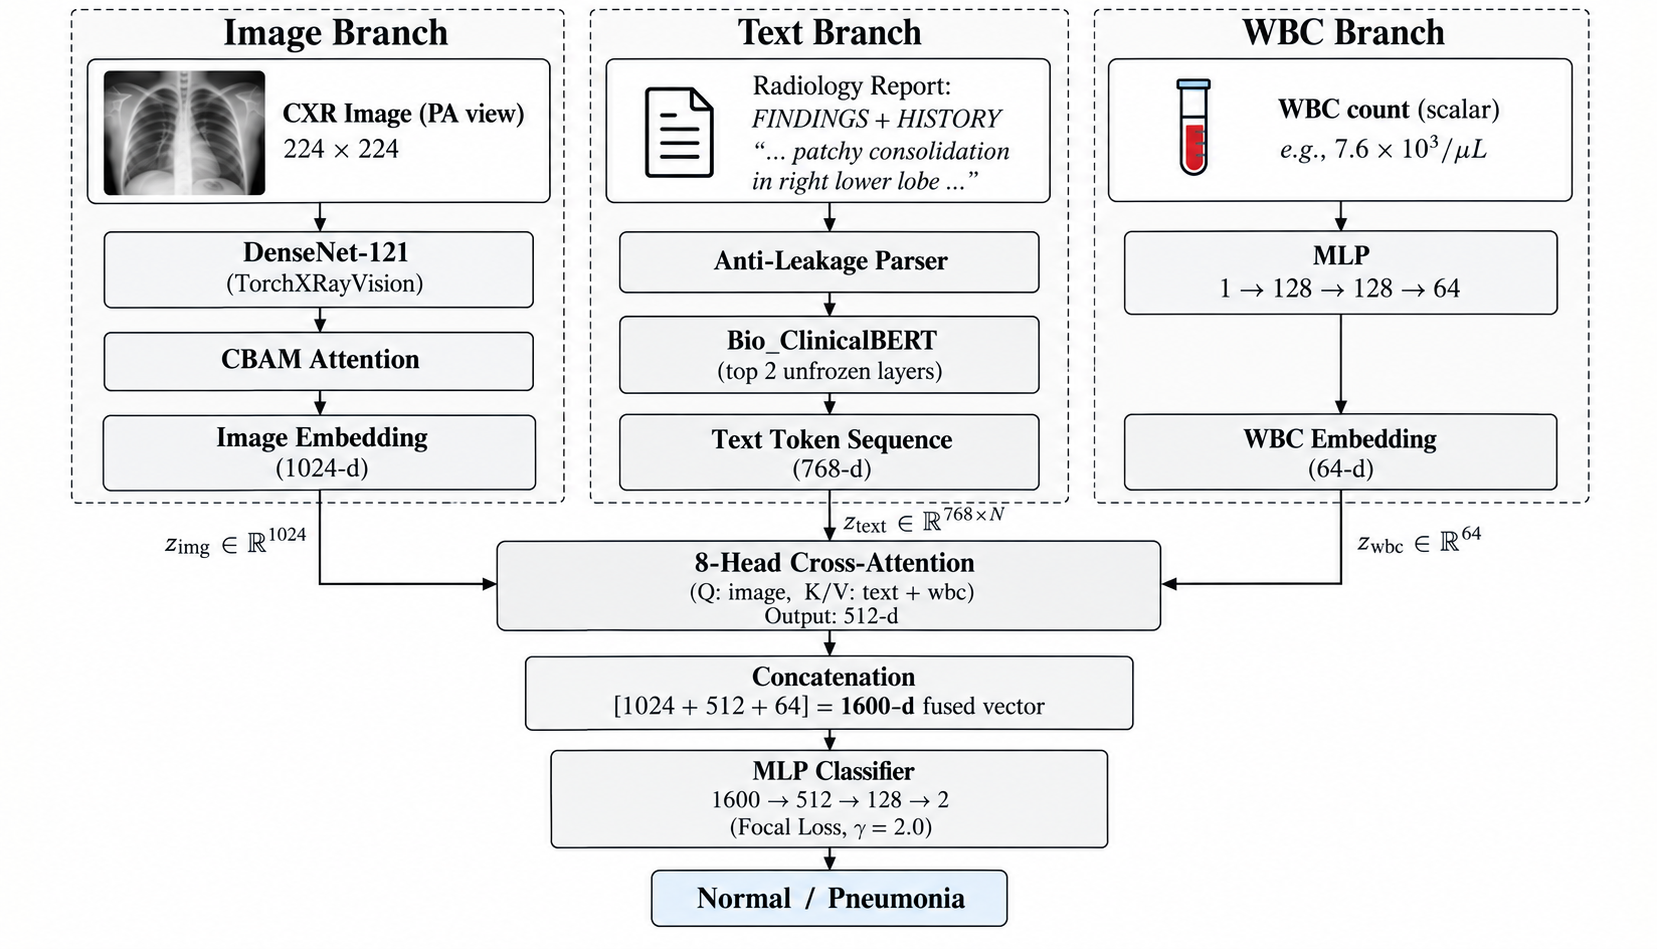
\includegraphics[width=0.85\textwidth]{architecture.png}
\caption{\textcolor{aideep}{PneumoFusionNet Phase~3c architecture.} Three input modalities---chest X-ray, leakage-free radiology report text, and WBC blood count---flow through separate encoder branches. The image and text representations interact via 8-head cross-attention, then concatenate with the WBC embedding to form a 1{,}600-dimensional feature vector for binary classification.}
\label{fig:architecture}
\end{figure*}

\subsection{Phase~1: Image Branch}

The image encoder employs \textbf{DenseNet-121}~\cite{huang2017densenet} pretrained on over 500{,}000 frontal chest radiographs via the TorchXRayVision~\cite{cohen2022torchxrayvision} library. Domain-specific pretraining is critical: pilot experiments showed that ImageNet-pretrained ResNet-50 failed to transfer to grayscale radiological textures (AUC dropped to 0.713 on scaled data).

A \textbf{Convolutional Block Attention Module (CBAM)}~\cite{woo2018cbam} is appended to the backbone to emphasise diagnostically relevant regions:
\begin{equation}
  \mathbf{M}_c(\mathbf{F}) = \sigma\!\left(\text{MLP}(\text{AvgPool}(\mathbf{F})) + \text{MLP}(\text{MaxPool}(\mathbf{F}))\right)
  \label{eq:channel}
\end{equation}
\begin{equation}
  \mathbf{M}_s(\mathbf{F}') = \sigma\!\left(f^{7\times7}\!\left([\text{AvgPool}_c(\mathbf{F}');\,\text{MaxPool}_c(\mathbf{F}')]\right)\right)
  \label{eq:spatial}
\end{equation}
where $\sigma$ denotes the sigmoid function and $r\!=\!16$ is the channel reduction ratio.

Training used 5-fold GroupKFold cross-validation with zero patient overlap, \textbf{Focal Loss}~\cite{lin2017focal} ($\gamma\!=\!2.0$), and 10-view Test-Time Augmentation (TTA). The output is a \textbf{1024-dimensional} image feature vector $\mathbf{v}_{\text{img}} \in \mathbb{R}^{1024}$, frozen for downstream phases.

\subsection{Phase~2: Radiology Text Fusion}

Radiology reports were preprocessed with a strict anti-leakage parser (detailed in Section~\ref{sec:antileak}) that retains only the HISTORY and FINDINGS sections while removing IMPRESSION/CONCLUSION and redacting diagnostic keywords.

Cleaned text is encoded using \textbf{Bio\_ClinicalBERT}~\cite{alsentzer2019bert}, pretrained on MIMIC-III clinical notes. The top two transformer layers (layers~10 and~11) are unfrozen with a conservative learning rate ($\eta_{\text{BERT}}\!=\!10^{-5}$) to enable task-specific adaptation while preventing catastrophic forgetting. The encoder emits the full token sequence $\mathbf{T} \in \mathbb{R}^{B \times 256 \times 768}$.

To capture cross-modal interactions, an \textbf{8-head cross-attention mechanism} allows image features to query relevant textual tokens:
\begin{equation}
  \mathbf{c}_{\text{cross}} = \text{softmax}\!\left(\frac{\mathbf{Q}_{\text{img}}\mathbf{K}_{\text{txt}}^\top}{\sqrt{d_k}}\right)\mathbf{V}_{\text{txt}}, \quad d_k = 64
  \label{eq:crossattn}
\end{equation}
where $\mathbf{Q}_{\text{img}} = \mathbf{v}_{\text{img}}\mathbf{W}_Q$ ($\mathbf{W}_Q \in \mathbb{R}^{1024 \times 512}$), $\mathbf{K}_{\text{txt}} = \mathbf{T}\mathbf{W}_K$, and $\mathbf{V}_{\text{txt}} = \mathbf{T}\mathbf{W}_V$ ($\mathbf{W}_K, \mathbf{W}_V \in \mathbb{R}^{768 \times 512}$). This produces $\mathbf{c}_{\text{cross}} \in \mathbb{R}^{512}$.

Training employs Focal Loss ($\gamma\!=\!2.0$) and embedding Mixup~\cite{zhang2018mixup} ($\alpha\!=\!0.2$) with differential learning rates: fusion head at $2\!\times\!10^{-4}$, BERT layers at $10^{-5}$.

\subsection{Phase~3c: WBC Fusion (Main Model)}

The WBC scalar value is transformed through a dedicated three-layer MLP rather than used as a raw input:
\begin{equation}
  \mathbf{e}_{\text{wbc}} = \text{MLP}(\text{wbc}): \; 1 \to 128 \to 128 \to 64
  \label{eq:wbcmlp}
\end{equation}
with ReLU activations and dropout (0.3, 0.2). This nonlinear projection is clinically motivated: a WBC of 12{,}000 vs.\ 16{,}000 vs.\ 28{,}000~cells/$\mu$L represents qualitatively different clinical states (borderline leukocytosis vs.\ severe acute infection) that a linear transformation cannot capture.

The final multimodal representation is formed by concatenating all three embeddings:
\begin{equation}
  \mathbf{z} = [\,\mathbf{v}_{\text{img}} \,\|\, \mathbf{c}_{\text{cross}} \,\|\, \mathbf{e}_{\text{wbc}}\,] \in \mathbb{R}^{1600}
  \label{eq:concat}
\end{equation}
where $\mathbf{v}_{\text{img}} \in \mathbb{R}^{1024}$, $\mathbf{c}_{\text{cross}} \in \mathbb{R}^{512}$, and $\mathbf{e}_{\text{wbc}} \in \mathbb{R}^{64}$, yielding a 1{,}600-dimensional fused vector.

The classifier head applies:
\begin{equation}
  \text{LayerNorm}(1600) \to \text{Dropout}(0.4) \to 512 \to 128 \to 2
  \label{eq:head}
\end{equation}
with GELU activations and progressive dropout (0.4, 0.3, 0.2).

\textbf{Warm-start protocol:} Phase~3c loads the trained cross-attention weights from the Phase~2 checkpoint, preserving cross-modal alignment while learning the WBC branch from scratch. Learning rates: BERT\,=\,$10^{-5}$, fusion head\,=\,$2\!\times\!10^{-4}$, WBC encoder\,=\,$10^{-3}$.

% ==========================================================
%  V. ANTI-LEAKAGE PROTOCOL
% ==========================================================
\section{\textcolor{aideep}{Anti-Leakage Protocol}}
\label{sec:antileak}

A critical concern in multimodal medical AI is diagnostic label leakage through text. Radiology reports contain an IMPRESSION section that directly states the diagnosis. Models trained on raw reports achieve artificially high performance by memorising this conclusion rather than learning from clinical evidence.

PneumoFusionNet enforces the following safeguards:
\begin{enumerate}[noitemsep, leftmargin=*]
  \item \textbf{Impression Removal:} IMPRESSION and CONCLUSION sections are stripped before tokenisation. Only FINDINGS and HISTORY are retained.
  \item \textbf{Keyword Redaction:} Diagnostic trigger words (e.g., ``pneumonia'', ``pneumonic'', ``compatible with'', ``normal study'') in remaining text are replaced with \texttt{[REDACTED]} via regular expressions.
  \item \textbf{Patient-Level Splitting:} All partitions enforce strict grouping on \texttt{subject\_id} (GroupKFold / GroupShuffleSplit) with automated verification: Train $\cap$ Val\,=\,$\emptyset$, Train $\cap$ Test\,=\,$\emptyset$, Val $\cap$ Test\,=\,$\emptyset$.
  \item \textbf{PA-Only Filtering:} AP views were removed after pilot experiments revealed that view type correlated with patient acuity, creating an acquisition-bias shortcut.
  \item \textbf{Train-Only Imputation:} Missing WBC values (15\%) are imputed using the training-set median; the same value is applied to validation and test partitions.
\end{enumerate}

% ==========================================================
%  VI. RESULTS
% ==========================================================
\section{\textcolor{aideep}{Results}}

All results are reported on held-out test sets with patient-level partitioning. Decision thresholds are optimised on the validation set using Youden's J statistic ($J = \text{TPR} - \text{FPR}$).

% ── Table I: Main Results ─────────────────────────────────
\begin{table}[t]
\centering
\caption{\textcolor{aideep}{Performance Across Modalities (Scale-Up Cohort)}}
\label{tab:results}
\setlength{\tabcolsep}{4pt}
\begin{tabular}{@{}lccccc@{}}
\toprule
\textbf{Phase / Model} & \textbf{Modality} & \textbf{AUC} & \textbf{Acc.} & \textbf{Sens.} & \textbf{Spec.} \\
\midrule
Phase 1 (CV)$^\dagger$ & CXR only & 0.826 & 76.3\% & 71.0\% & 81.6\% \\
Phase 2v2$^\ddagger$ & CXR + Text & 0.946 & 87.8\% & 86.6\% & 89.1\% \\
\textbf{Phase 3c}$^\S$ & \textbf{CXR + Text + WBC} & \textbf{0.971} & \textbf{92.9\%} & \textbf{92.3\%} & \textbf{93.6\%} \\
\bottomrule
\multicolumn{6}{@{}l}{\footnotesize $^\dagger$5-fold GroupKFold mean (AUC $0.826 \pm 0.017$, $N$=3{,}763).}\\
\multicolumn{6}{@{}l}{\footnotesize $^\ddagger$Youden-J threshold ($\tau$=0.568), $N_{\text{test}}$=582.}\\
\multicolumn{6}{@{}l}{\footnotesize $^\S$Youden-J threshold ($\tau$=0.559), $N_{\text{test}}$=565.}\\
\end{tabular}
\end{table}

Table~\ref{tab:results} presents the progressive performance across modalities. The image-only model exhibited a ceiling at AUC\,=\,0.826 despite extensive optimisation (5-fold CV, TTA, CBAM, Focal Loss). Incorporating leakage-free radiology text resulted in a substantial +12.0 percentage point AUC gain. Adding the WBC scalar further increased AUC to 0.971, with notable improvements in both sensitivity (+5.6pp) and specificity (+4.5pp).

% ── Table II: Threshold Analysis ──────────────────────────
\begin{table}[t]
\centering
\caption{\textcolor{aideep}{Phase~3c Operating Threshold Analysis ($N_{\text{test}}$=565)}}
\label{tab:thresholds}
\setlength{\tabcolsep}{3.5pt}
\begin{tabular}{@{}lcccc@{}}
\toprule
\textbf{Strategy} & \textbf{Threshold} & \textbf{Acc.} & \textbf{Sens.} & \textbf{Spec.} \\
\midrule
Default ($\tau$=0.50) & 0.500 & 92.4\% & \textbf{94.7\%} & 90.0\% \\
Youden-J (Optimal) & 0.559 & \textbf{92.9\%} & 92.3\% & 93.6\% \\
Clinical Target & 0.575 & 92.7\% & 91.2\% & \textbf{94.3\%} \\
\bottomrule
\end{tabular}
\end{table}

Table~\ref{tab:thresholds} shows the operating characteristics of Phase~3c under three threshold strategies. The default threshold maximises sensitivity (94.7\%), suitable for emergency triage where missed pneumonia cases carry high clinical cost. The Youden-J threshold provides optimal balanced performance, while the clinical target threshold achieves maximum specificity while maintaining sensitivity above 90\%.

% ── Figure: ROC Curve ─────────────────────────────────────
\begin{figure}[t]
  \centering
  
\includegraphics[width=\columnwidth]{p3c_roc_curve.png}
  \caption{\textcolor{aideep}{ROC curve for Phase~3c} (CXR + Text + WBC) on the held-out test set ($N$=565), achieving AUC\,=\,0.971.}
  \label{fig:roc}
\end{figure}

% ── Figure: Pipeline Comparison ───────────────────────────
\begin{figure}[t]
  \centering
  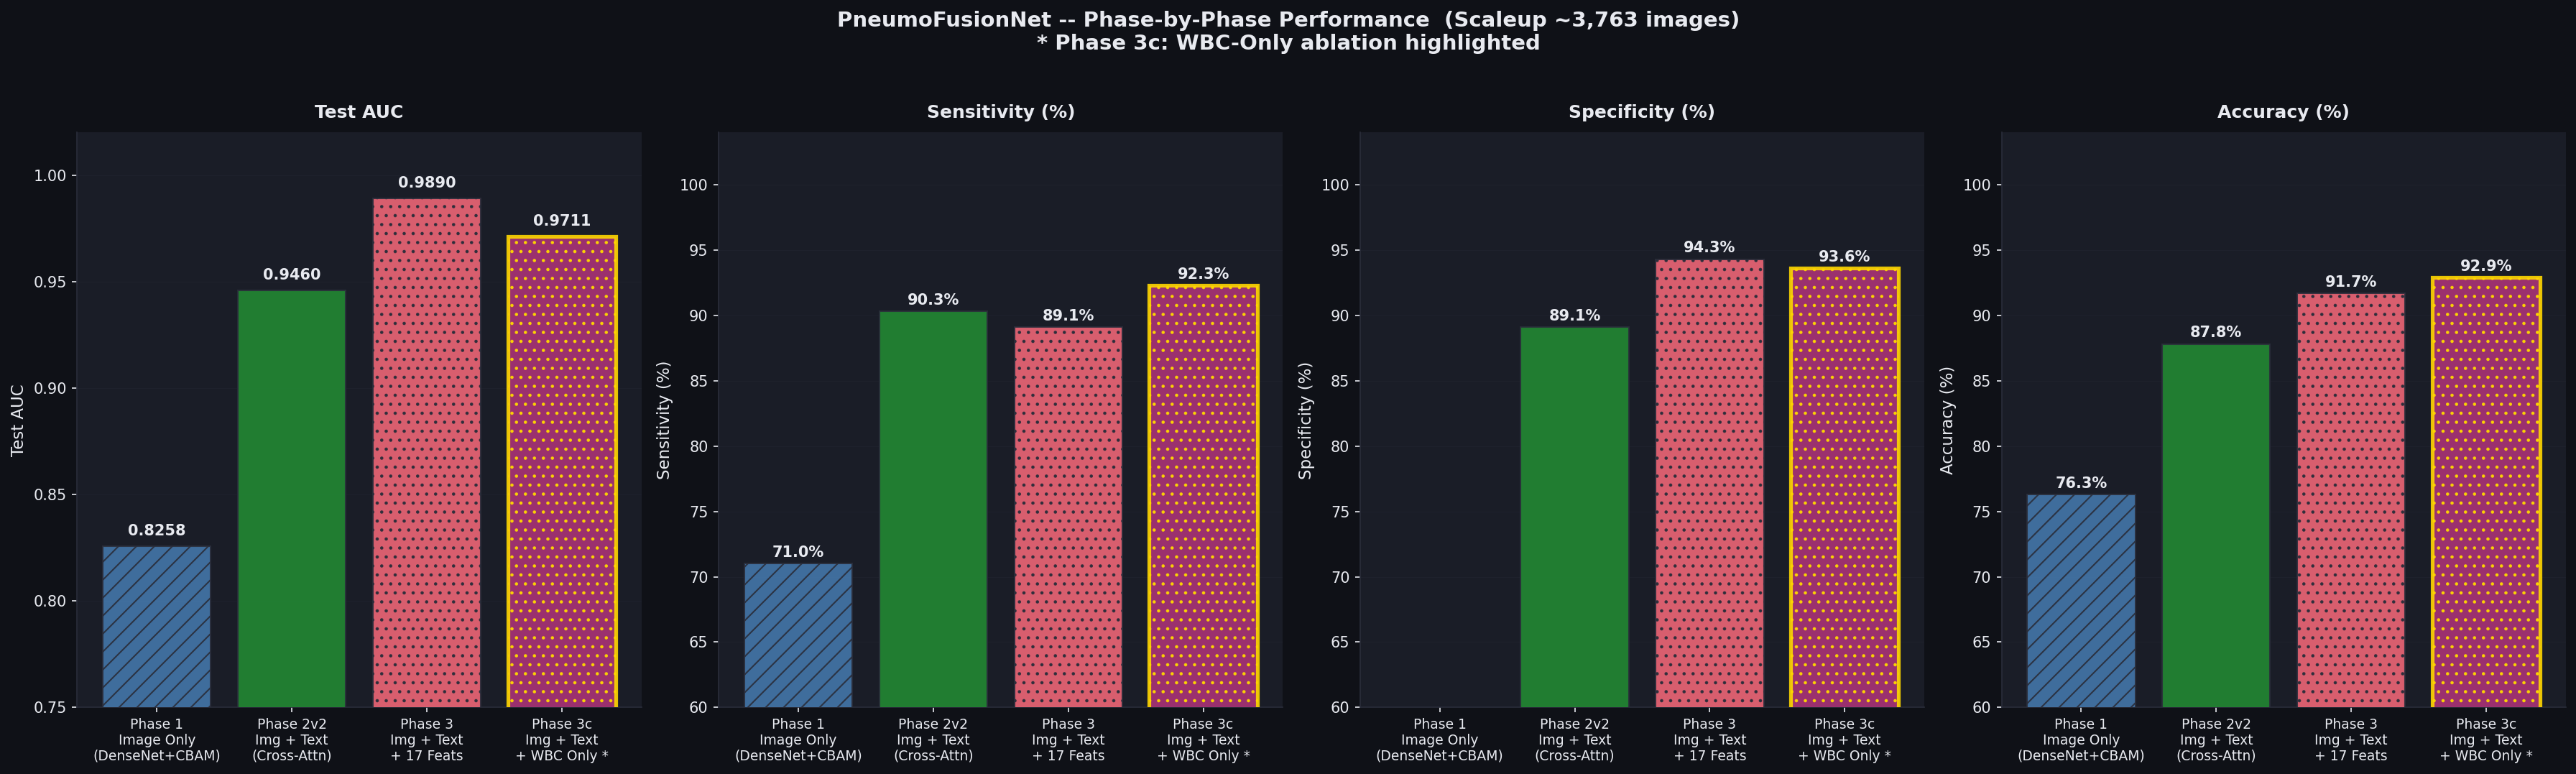
\includegraphics[width=\columnwidth]{p3c_full_pipeline_comparison.png}
  \caption{\textcolor{aideep}{Progressive pipeline comparison} showing AUC, accuracy, sensitivity, and specificity gains across Phase~1 (Image only), Phase~2 (Image + Text), and Phase~3c (Image + Text + WBC).}
  \label{fig:pipeline}
\end{figure}

% ==========================================================
%  VII. DISCUSSION
% ==========================================================
\section{\textcolor{aideep}{Discussion}}

Several key observations emerge from this study:

\textbf{Multimodal learning substantially outperforms image-only approaches.} The image-only model plateaued at AUC\,=\,0.826 despite extensive architectural optimisation. This ceiling exists because chest radiographs depict anatomical structure but cannot reveal the patient's physiological state---fever duration, immune activation, or clinical history.

\textbf{Cross-attention enables effective image-text alignment.} The 8-head cross-attention mechanism allows image features to selectively attend to relevant textual tokens. When the radiograph shows an ambiguous opacity, the model can attend to descriptive terms such as ``consolidation'', ``fever'', or ``productive cough'' in the report, disambiguating pathology from benign findings.

\textbf{Strict anti-leakage is essential for valid evaluation.} Removing the IMPRESSION section and redacting diagnostic keywords ensures that observed performance gains reflect genuine multimodal learning rather than direct access to diagnostic labels.

\textbf{A single laboratory biomarker provides substantial diagnostic value.} Although WBC is only one scalar measurement, its integration contributed meaningful improvements: +2.5pp AUC, +5.6pp sensitivity, and +4.5pp specificity over image-text fusion alone. A Complete Blood Count providing WBC results is a universal, point-of-care test available within 15~minutes of patient presentation, making the CXR\,+\,Report\,+\,WBC triad feasible within 30~minutes of emergency admission.

\textbf{Comparison with full clinical panel:} A separate experiment integrating 17 clinical features (demographics, vital signs, and laboratory values) achieved AUC\,=\,0.969 but with \emph{lower} sensitivity (89.1\% vs.\ 92.3\%) and required 1--4~hours of laboratory processing. Phase~3c with WBC alone achieves comparable discrimination with higher sensitivity and dramatically faster turnaround.

\textbf{Limitations.} All data originate from a single US institution (Beth Israel Deaconess Medical Centre). The binary classification formulation does not address multi-label co-morbidities. Approximately 15\% of WBC values required median imputation. External validation on diverse populations and scanner hardware is necessary.

% ==========================================================
%  VIII. CONCLUSION
% ==========================================================
\section{\textcolor{aideep}{Conclusion}}

This work presented PneumoFusionNet, a leakage-controlled multimodal framework that integrates chest radiographs, radiology report text, and White Blood Cell count for pneumonia detection. The proposed approach achieved progressive improvements from image-only learning (AUC\,=\,0.826) to image-text fusion (AUC\,=\,0.946) and finally image-text-WBC fusion (AUC\,=\,0.971, Sensitivity\,=\,92.3\%, Specificity\,=\,93.6\%).

The findings demonstrate that combining complementary clinical modalities substantially improves diagnostic performance while maintaining a realistic evaluation protocol. The CXR\,+\,Report\,+\,WBC triad can be evaluated within 30~minutes of emergency admission, making the framework directly applicable to clinical workflows.

Future work will investigate external validation on Indian hospital datasets with different patient demographics and scanner hardware, multi-label classification for co-occurring pathologies, additional laboratory biomarkers, and transformer-based multimodal fusion architectures.

\vspace{4pt}
\noindent\textbf{Code and Data:} \url{https://github.com/Ashutosh-yadav0001/PneumoFusionNet}. MIMIC-CXR data requires PhysioNet credentialled access (CITI training and DUA).

% ==========================================================
%  REFERENCES
% ==========================================================
{\small
\begin{thebibliography}{11}

\bibitem{who2023}
World Health Organization, ``Pneumonia,'' \emph{WHO Fact Sheet}, 2023.
\url{https://www.who.int/news-room/fact-sheets/detail/pneumonia}

\bibitem{rajpurkar2017chexnet}
P.~Rajpurkar et~al., ``CheXNet: Radiologist-Level Pneumonia Detection on Chest X-Rays with Deep Learning,'' \emph{arXiv:1711.05225}, 2017.

\bibitem{frontiers2025pneumofusion}
S.~Yu et~al., ``A multi-modal deep learning solution for precise pneumonia diagnosis: the PneumoFusion-Net model,'' \emph{Frontiers in Physiology}, vol.~16, Art.~1512835, Mar.\ 2025.

\bibitem{johnson2019mimic}
A.~E.~W.~Johnson et~al., ``MIMIC-CXR, a de-identified publicly available database of chest radiographs with free-text reports,'' \emph{Scientific Data}, vol.~6, no.~317, 2019.

\bibitem{johnson2023mimiciv}
A.~E.~W.~Johnson et~al., ``MIMIC-IV, a freely accessible electronic health record dataset,'' \emph{Scientific Data}, vol.~10, no.~1, p.~1, 2023.

\bibitem{alsentzer2019bert}
E.~Alsentzer et~al., ``Publicly Available Clinical BERT Embeddings,'' \emph{arXiv:1904.03323}, 2019.

\bibitem{huang2017densenet}
G.~Huang, Z.~Liu, L.~van~der~Maaten, and K.~Q.~Weinberger, ``Densely Connected Convolutional Networks,'' \emph{Proc.\ IEEE CVPR}, 2017, pp.~4700--4708.

\bibitem{woo2018cbam}
S.~Woo, J.~Park, J.-Y.~Lee, and I.~S.~Kweon, ``CBAM: Convolutional Block Attention Module,'' \emph{Proc.\ ECCV}, 2018, pp.~3--19.

\bibitem{lin2017focal}
T.-Y.~Lin, P.~Goyal, R.~Girshick, K.~He, and P.~Doll{\'a}r, ``Focal Loss for Dense Object Detection,'' \emph{Proc.\ IEEE ICCV}, 2017, pp.~2980--2988.

\bibitem{zhang2018mixup}
H.~Zhang, M.~Ciss{\'e}, Y.~N.~Dauphin, and D.~Lopez-Paz, ``Mixup: Beyond Empirical Risk Minimization,'' \emph{Proc.\ ICLR}, 2018.

\bibitem{cohen2022torchxrayvision}
J.~P.~Cohen et~al., ``TorchXRayVision: A Library of Chest X-Ray Datasets and Models,'' \emph{Proc.\ MICCAI Workshop on Medical Imaging with Deep Learning}, 2022.

\end{thebibliography}
}

\end{document}
